\section{Introduction} 

Fluid-elastic galloping is one of the sub-areas of research in fluid structure interactions. This area has been of interest due to the vibrations crated by galloping on transmission lines and civil structures and leading them to failure. Therefore understanding this phenomenon in order to suppresses these vibrations was quite important. However, the search for alternate energy sources with minimal environmental impact has become an important area of research in the modern word. Therefore researchers are moving towards investigating the possibility of extracting useful energy from this vibrations rather than suppressing them. Thus, it is quite important to understand the governing parameters and analyse the influence of them on the energy transfer from the fluid to the structure, because this understanding will lead to develop better practical applications. Hence, in this paper we focus on understanding the energy transfer from the fluid to the body and isolate the governing parameters influencing it.

According to \citet{Paidoussis2010}, \citet{Glauert1919} provided a criterion for galloping by considering the auto-rotation of an aerofoil.  \citet{DenHartog1956} provided a theoretical explanation for galloping for iced electric transmission lines. A weakly non-linear theoretical aeroelastic model to predict the response of galloping was developed by \citet{Parkinson1964} based on the quasi-steady state hypothesis. Experimental lift and drag data on a fixed square prism at different angles of attack were used as an input for the theoretical model. It essentially used a curve fit of the transverse force to predict the galloping response. The study managed to achieve a good agreement with experimental data.

However, the QSS model equation when solved analytically using the sinusoidal solution method cannot predict the response for cases with low mass ratios. \citet{Joly2012} observed that finite element simulations show a sudden change in amplitude below a critical value of the mass ratio. The quasi-oscillator equation in \citet{Parkinson1964} was altered to account for the vortex shedding and solved numerically to predict the reduced amplitude at low mass ratios to the point where galloping is no longer present. \citet{Barrero-Gil2010a} investigated the possibility of extracting power from vibrations caused by galloping using the quasi-steady state model. In the conclusions of that paper it was pointed out that in order to obtain a high power to area ratio, the mass-damping ($m^*\zeta$) parameter should be kept low. The same study investigated the influence of the characteristics of the $C_y$ curve on maximum power output.

Here, the modified QSS model developed by \citet{Joly2012} is integrated numerically for low Reynolds numbers. The focus is on the power transfer from the fluid to the structure and the influence of mechanical parameters (i.e. frequency of oscillation, damping factor and mass ratio). To this end, a series of previously mentioned mechanical parameters are tested at two different values of \reynoldsnumber: $\reynoldsnumber = 165$, a case that should remain laminar and essentially two-dimensional; $\reynoldsnumber = 22300$, a case where the flow is expected to be turbulent and three-dimensional. Both cases require the input of transverse force coefficients $C_y$ as a function of angle of attack $\theta$ for a fixed body. These data are provided from direct numerical simulations for the $\reynoldsnumber = 165$ case, while the data provided by \citet{Parkinson1964} are used for the $\reynoldsnumber = 22300$ case.

The structure of the paper is as follows. Section \ref{sec:theory} presents the governing equations and the oscillator model used to obtain data, the method for the calculation of the power transferred from the fluid to the structure. The governing parameters namely, the combined mass-stiffness and the combined mass-damping obtained using linearised time scales of the oscillator model are also being introduced. Section \ref{sec:results} presents the results, first of the fixed body tests at a range of $\theta$, then of the response characteristics predicted by the integration of the QSS model for both the high and low \reynoldsnumber\ cases. For the low \reynoldsnumber\ case, the results of the QSS model are compared to those of full direct numerical simulations of the fluid-structure interaction problem. Finally, section \ref{sec:conc} presents the conclusions that can be drawn from this work.
% % % % % % % % % % % % % % % % % % % % % % % % % % % % % % % % % % % % % % % % % % % % % % % % % % % % % % % % % % % % % % % % % % % % % % % % 
\section*{Nomenclature}
%\textbf{Nomenclature}

\begin{tabular}{ll}
$a_1,a_3,a_5,a_7$ & coefficients of the polynomial to determine $C_y$ \\ 
$A$ & displacement amplitude\\
$c$ & damping constant \\
$D$ & characteristic length (side length) of the cross section of the body \\
$f=\sqrt{k/m}/2\pi$ & natural frequency of the system \\
$F_y$ & instantaneous force normal to the flow \\ 
$F_0$& amplitude of the oscillatory force due to vortex shedding \\
$k$ & spring constant \\
$m$ & mass of the body \\
$m_a$ & added mass \\
$P_d$ & power dissipated due to mechanical damping  \\
$P_{in}=\rho U^3D/2$ & Energy flux of the approaching flow \\
$P_{mean}$ & mean power \\
$P_t$   & power transferred to the body by the fluid \\
$t$ & time \\
$U$ & freestream velocity \\
$U_i$ & Induced velocity \\
$y,\dot{y},\ddot{y}$ & transverse displacement, velocity and acceleration of the body \\
$\mathcal{A}=DL$ & frontal area of the body\\ 
$\lambda$ & Inverse time scale of a galloping dominated flow \\
$\lambda_{1,2}$ & Eigenvalues of linearized equation of motion \\
$\rho$ & fluid density  \\
$\omega_n= 2 \pi f$ & natural angular frequency of the system  \\
$\omega_s$ & vortex shedding angular frequency \\
$\cstar=cD/mU$ & non-dimensionalised damping factor \\
$C_y=F_y/0.5\rho U^2DL$ & normal (lift) force coefficient \\
$m^*=m/\rho D^2L$ & mass ratio \\
$Re$ & Reynolds number  \\
$U^*=U/fD$ & reduced velocity  \\
$Y=y/D$ & non-dimensional transverse displacement \\
$\dot{Y}=m^*\dot{y}/a_1U$ & non-dimensional transverse velocity \\
$\ddot{Y}=m^{*2}D/a_1^2U^2$ & non-dimensional transverse acceleration \\
$\Gamma_1 = 4\pi^2m^{*2}/U^{*2}a_1^2$ & First dimensionless group arising from linearised, non-dimensionalised equation of motion\\
$\Gamma_2 = c^*m^*/a_1$ & Second dimensionless group arising from linearised, non-dimensionalised equation of motion\\
$\zeta= c/2 m \omega_n$ & damping ratio \\
$\theta= \tan^{-1}{(\dot{y}/U)}$ & instantaneous angle of incidence (angle of attack)\\
$\massstiff =  4\pi^2m^{*2}/U^{*2}$ & Combined mass-stiffness parameter\\
$\massdamp = c^*m^*$ & Combined mass-damping parameter\\
\end{tabular}  


% % % % % % % % % % % % % % % % % % % % % % % % % % % % % % % % % % % % % % % % % % % % % % % % % % % % % % % % % % % % % % % % % % % % % % % % % % % %

\section{Problem formulation and methodology}
\label{sec:theory}

\subsection{The quasi-steady state (QSS) model}

The equation of motion of the body is given by 
\begin{equation}
\label{equationofmotion}
(m+m_a)\ddot{y}+c\dot{y}+ky=F_y,
\end{equation}
where the forcing term $F_y$ is given by
\begin{equation}
\label{lift equation}
F_y=\frac{1}{2}\rho U^2\mathcal{A}C_y.
\end{equation}
\citet{lighthill1986} showed that for systems oscillating in fluid, it is sometimes useful to decompose the fluid forces into components that are in and out of phase with the body acceleration. The component in phase with the acceleration effectively adds to the inertia or effective mass of the system. Therefore, an added mass term, $m_a$, can be added to the system mass. For consistency with previous studies such as \citet{Joly2012}, a value of $m_a=3.5$ has been used here.

\begin{figure}
\setlength{\unitlength}{\textwidth}

  \begin{picture}(1,0.23)(0,0.74)
    
  \put(0.2,0.76){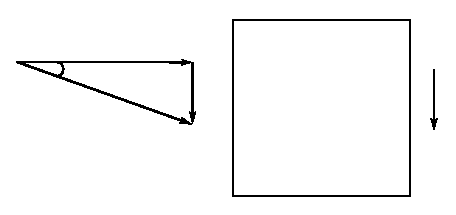
\includegraphics[width=0.5\unitlength]{../FnP/gnuplot/setup-1.eps}}         
      
      
   
 	\put(0.315,0.93){$U$}
 	\put(0.3,0.84){$U_i$}
    \put(0.42,0.88){$\dot{y}$}
    \put(0.28,0.895){ $\theta$}
    \put(0.7,0.87){\small $(+)$}
      	

 	
 	 

     

  \end{picture}

 \caption{Induced angle of attack on the square prism due to the resultant of free-stream velocity of the fluid and transverse velocity of the body.}
    \label{fig:setup_1}
\end{figure}

In the QSS model, it is assumed that the force on the body at a given instantaneous incident angle $\theta$ (defined in figure \ref{fig:setup_1}) is the same as the mean force on a static body at the same incident angle, or angle of attack. The instantaneous value of $C_y$ is therefore determined by an interpolating polynomial based on the lift data for flow over a stationary body at various $\theta$. Using the relationship between $\theta$ and the instantaneous transverse velocity of the body $\dot{y}$ shown in figure \ref{fig:setup_1}, $C_y$ can be written as a function of $\dot{y}$. The order of the interpolation polynomial used to define this function has varied from study to study. For  example a $7^{th}$ order polynomial was used in \cite{Parkinson1964} and $3^{rd}$ order polynomial was used in \cite{Barrero-Gil2009}. \cite{Ng2005} concluded that using a $7^{th}$ order polynomial is sufficient and a polynomial higher than that of $7^{th}$ order doesn't provides a significantly better result. Thus a $7 ^{th}$ order interpolating polynomial is used in this present study. As a result, $C_y(\theta)$ (noting that theta is proportional to $\dot{y}/U$) is defined as
\begin{equation}
\label{cy ploynomial}
C_y(\theta)=a_1\left(\frac{\dot{y}}{U}\right)+a_3\left(\frac{\dot{y}}{U}\right)^3+a_5\left(\frac{\dot{y}}{U}\right)^5+a_7\left(\frac{\dot{y}}{U}\right)^7.
\end{equation}

%\begin{equation}
%\label{modified_equation_of_motion}
%\ddot{y}+c^*\dot{y}+k^*y=\frac{1}{2}\rho U^2A
%\end{equation}

 It is expected that vortex shedding will be well correlated along the span and provide significant forcing at low \reynoldsnumber. \citet{Joly2012} introduced  an additional sinusoidal forcing function to the hydrodynamic forcing to model this. This enables the model to provide accurate predictions even at low mass ratios where galloping excitation is suppressed or not present. In this study, the forcing due to vortex shedding in low \reynoldsnumber\ cases is incorporated using a sinusoidal forcing function $F_0\sin{\omega_{s}t}$ added to the right-hand side of equation \ref{equationofmotion}. Here, $\omega_{s}$ and $F_0$ represent the angular vortex shedding frequency and the maximum force due to shedding respectively. Thus, the final equation for the modified QSS model is

\begin{equation}
\label{final_equation_motion}
m\ddot{y}{+}c\dot{y}{+}ky{=}\frac{1}{2}\rho U^2 \mathcal  {A} \Bigg(a_1\left(\frac{\dot{y}}{U}\right){+}a_3\left(\frac{\dot{y}}{U}\right)^3{+}a_5\left(\frac{\dot{y}}{U}\right)^5{+}a_7\left(\frac{\dot{y}}{U}\right)^7 \Bigg){+} F_0\sin{(\omega_s t)}.
\end{equation}

This equation can be solved using standard time integration methods. In this study the fourth-order Runge-Kutta scheme built in to the MATLAB routine `ode45' was generally used to obtain the solutions. Some low mass ratio cases used a solver modified for stiff problems, built into the `ode15s' routine in MATLAB.

\subsection{Calculation of average power}

 The dissipated power due to the mechanical damping represents the ideal potential amount of harvested power output. Therefore, the mean power output can be given by
\begin{equation}
\label{power}
P_{mean}=\frac{1}{T}\int_{0}^{T}(c\dot{y})\dot{y} dt,
\end{equation}
where $T$ is the period of integration and $c$ is the mechanical damping constant. 

It should be noted that this quantity is equal to the work done on the body by the fluid, defined as
\begin{equation}
\label{power_alt}
P_{mean}=\frac{1}{T}\int_{0}^{T}F_y\dot{y} dt,
\end{equation}
where $F_y$ is the transverse (lift) force.

These two definitions show two important interpretions of the power with respect to any energy production device. The first shows that power will be high for situations where the damping coefficient is high, and the transverse velocity is consistently high. The second shows that power will be high for situations where the transverse force and the body velocity are in phase.
 
 \begin{figure}

  \setlength{\unitlength}{\textwidth}
  \begin{picture}(1,0.25)(0,0.8)
  
    % % %90
      \put(0.025,0.81){\includegraphics[width=0.5\unitlength]{../FnP/gnuplot/lift_curve_165.eps}}
      \put(0.495,0.81){\includegraphics[width=0.5\unitlength]{../FnP/gnuplot/lift_curve_park.eps}}
 	\put(0.02,0.93){ \large $C_y$} 	
% 	\put(0.56,1.02){ $\theta$}
 	
        \put(0.25,0.8){ $\theta$} 	
        \put(0.75,0.8){ $\theta$}
        
        \put(0.105,1.01){(a)}
        \put(0.565,1.01){(b)}
      \end{picture}

  \caption{Lift coefficient, $C_y$, as a function of incidence angle $\theta$, for a static square cross section. (a) Data from simulations at $Re=165$  (b) data from \cite{Parkinson1964} at $Re=22300$. Points ($\bullet$) are measurements from the simulations. The solid lines in both plots are 7th-order interpolating polynomial used to predict the fluid forcing for the QSS model.}
    \label{fig:lift_curves}
\end{figure}

 \begin{table}[ht]

\begin{center}
\setlength{\unitlength}{\textwidth}

\begin{tabular}{c c c c c} % centered columns (4 columns)
\hline\hline %inserts double horizontal lines
\\[0.2ex]
Case & $a_1$ & $a_3$ & $a_5$ & $a_7$ \\ [0.8ex] % inserts table 
%heading
\hline 
\\[0.8ex]% inserts single horizontal line
Re=165 & 1.3 & 125.3 & 1825.73 & 8765.3 \\[0.8ex] % inserting body of the table
Re=22300 & 2.69 & 168 & 1670 & 59900 \\ [1ex] % [1ex] adds vertical space
\hline %inserts single line
\end{tabular}

\caption{Coefficient values used in the 7th order interpolation polynomial for high ($Re=22300$) and low ($Re=165$) Reynolds numbers. These data are used as input data to calculate the RHS of Eq.\ref{final_equation_motion} throughout this study.}
 
\label{table:nonlin} % is used to refer this table in the text
\end{center}
\end{table}


 
 
 % % % % % % % % % % % % % Time scales % % % % % % % % % % % % % % % % % % % % % % % % % % % % % % %
 The natural time scales of the system can be found by solving for the eigenvalues of the linearized equation of motion, namely
 \begin{equation}
 \label{eqn:eom_linear}
 (m+m_a)\ddot{y}{+}c\dot{y}{+}ky{=}\frac{1}{2}\rho U^2 \mathcal{A} a_1\left(\frac{\dot{y}}{U}\right),
 \end{equation}
 which is simply the equation of motion presented in equation \ref{final_equation_motion} with the polynomial series for the lift force truncated at the linear term, and the forcing term representing vortex shedding removed.
 
 Combining the $\dot{y}$ terms and solving for eigenvalues gives
 \begin{equation}
   \label{eqn:eigs}
   \lambda_{1,2}= -\frac{1}{2}\frac{c-\frac{1}{2}\rho U\mathcal{A}a_1}{(m+m_a)}\pm\frac{1}{2}\sqrt{\left[\frac{c-\frac{1}{2}\rho U\mathcal{A}a_1}{(m+m_a)}\right]^2-4\frac{k}{(m+m_a)}}.
 \end{equation}
 
 If it is assumed that the spring is relatively weak, $k\rightarrow 0$, a single non-zero eigenvalue remains. This eigenvalue is
 \begin{equation}
   \label{eqn:eigs_nospring}
   \lambda=-\frac{c-\frac{1}{2}\rho U\mathcal{A}a_1}{(m+m_a)}.
 \end{equation}
 
 Further, if it is assumed that the mechanical damping is significantly weaker than the aerodynamic forces on the body, $c\rightarrow 0$ and
 \begin{equation}
   \label{eqn:eigs_nospring_nodamp}
   \lambda=\frac{\frac{1}{2}\rho U\mathcal{A}a_1}{(m+m_a)}.
 \end{equation}
 
 For reasonably heavy bodies, the impact of the added mass can also be neglected, to arrive at a definition of $\lambda$ as
 \begin{equation}
   \label{eqn:eigs_nospring_nodamp}
   \lambda=\frac{\frac{1}{2}\rho U\mathcal{A}a_1}{m}.
 \end{equation}
 
 In this form, $\lambda$ represents the inverse time scale of the motion of the body due to the negative damping effect of the long-time aerodynamic forces. In fact, the terms can be regrouped and $\lambda$ written as
 \begin{equation}
   \label{eqn:timescale}
   \lambda = \frac{a_1}{m^*}\frac{U}{D}
 \end{equation}
 
 Written this way, the important parameters that dictate this inverse time scale are clear. The rate of change in the aerodynamic force with respect to angle of attack when the body is at the equilibrium position, $\partial C_y/\partial \alpha$, is represented by $a_1$. The mass ratio is represented by $m^*$. The inverse advective time scale of the incoming flow is represented by the ratio $U/D$. Increasing $a_1$ would mean the force on the body would increase more rapidly with small changes in the angle of attack, $\theta$, or transverse velocity. Equation \ref{eqn:timescale} shows that such a change will increase the inverse time scale, or analogously decrease the response time of the body. Increasing the mass of the body, thereby increasing $m^*$, has the opposite effect. The inverse time scale is decreased, or as might be expected, a heavier body will take longer to respond.
 
 This timescale can then be used to non-dimensionalize the equation of motion, and to find the relevant dimensionless groups of the problem. If the non-dimensional time, $\tau$, is defined such that $\tau=t(a_1/m^*)(U/D)$, the equation of motion presented in equation \ref{final_equation_motion} can be non-dimensionalized as
 \begin{equation}
   \label{eqn:eom_nondim}
   \ddot{Y} + \frac{m^{*2}}{a_1^2}\frac{kD^2}{mU^2}Y = \left(\frac{1}{2} - \frac{m^*}{a_1}\frac{cD}{mU}\right)\dot{Y} + H.O.T.,
 \end{equation}
 
 where $H.O.T.$ respresents the higher order terms in $\dot{Y}$. The coefficients can be regrouped into combinations of non-dimensional groups, and rewritten as
 \begin{equation}
   \label{eqn:eom_nondim_regroup}
   \ddot{Y} + \frac{4\pi^{2}m^{*2}}{U^{*2}a_1^2}Y = \left(\frac{1}{2} - \frac{c^*m^*}{a_1}\right)\dot{Y} + H.O.T,
 \end{equation}
 
 where $c^*=cD/mU$ is a non-dimensional damping parameter.
 
 Equation \ref{eqn:eom_nondim_regroup} shows there are four non-dimensional parameters that play a role in setting the response of the system. These are the stiffness (represented by the reduced velocity $U^*$), the damping $c^*$, the mass ratio $m^*$, and the geometry, represented by the rate of change in the aerodynamic force with respect to angle of attack when the body is at the equilibrium position, $a_1$. The grouping of these parameters into two groups in equation \ref{eqn:eom_nondim_regroup} which arise by non-dimensionalising using the natural time scale of the galloping system, suggests there are two groups that dictate the response: $\Gamma_1 = 4\pi^2m^{*2}/U^{*2}a_1^2$ and $\Gamma_2 = c^*m^*/a_1$. For a given geometry and Reynolds number, $\Gamma_1$ can be thought of as a combined mass-stiffness, whereas $\Gamma_2$ can be thought of a a combined mass-damping parameter. As it is assumed that during galloping the stiffnes plays only a minor role, $\Gamma_2$ seems a likely parameter to collapse the data presented in figure \ref{fig:uncollapsed_data}. In fact, in the classic paper on galloping from \citet{Parkinson1964}, galloping data from wind tunnel tests is presented in terms of a parameter that can be shown to be the same as $\Gamma_2$.
 
 All of the quantities that make up $\Gamma_1$ and $\Gamma_2$ can, in theory, be known before an experiment is conducted. However, the quantity $a_1$ is a relatively difficult one to determine, requiring static body experiments or simulations. Here, the geometry is unchanged and results are only being compared at the same \reynoldsnumber. Hence, suitable parameters can be formed by multiplying $\Gamma_1$ and $\Gamma_2$ by $a_1^2$ and $a_1$ respectively, to arrive at a mass-stiffness parameter $\massstiff =  4\pi^2m^{*2}/U^{*2}$, and a mass-damping parameter defined as $\massdamp = c^*m^*$.
 
 
 
 
 
 
 
 
 
 
 
 
 
 
 
 
 
 
 
 
 
 
 
 
 
 
 
 
 
 
 
 
 
\subsection{Parameters used} 
 
For the low \reynoldsnumber\ tests, $\reynoldsnumber=165$ was maintained as it was pointed out by \citet{Sheard2009} and \citet{Tong2008} that the three-dimensional transition for a square cylinder occurs at approximately \reynoldsnumber=160. $F_0$ was kept at $0.4937$ which was obtained by scaling the value used by \citet{Joly2012} with the amplitude ratios of the lift forces obtained at the different Reynolds numbers. 

The angular vortex shedding frequency $\omega_s$, was set to $0.98$ which was obtained by performing a power spectral analysis of the stationary data at $0^\circ$. Stationary $C_y$ data were obtained at different angles of attack ranging from $0^\circ$ to $16^\circ$. The average power was obtained by using equation \ref{power}, and the averaging was done over no less than 20 galloping periods. Predictions of power output at $\reynoldsnumber=22300$ were obtained using the coefficients for curve fitting $C_y$ (Table (\ref{table:cy-coefficients})) from \citet{Parkinson1964}, in order to provide a comparison between high and low Reynolds numbers. The mass ratio $m^*$ was kept at 1163 for $\reynoldsnumber=22300$ (Similar to \citet{Parkinson1964}) and $m^*=20$ for \reynoldsnumber=165. These parameters were used throughout this study unless otherwise specified. 

The stationary data and the fluid-structure interaction (FSI) data were obtained using a high-order spectral element routine to simulate the two-dimensional laminar flow.  Simulations involving fluid structure interaction (FSI) were used to provide additional validation of the QSS model. The inlet was placed $20D$ while the outlet situated $60D$ away from the centroid of the body. The side boundaries were placed $20D$ away from the centroid of the body where $D$ was kept as unity throughout this study. The Navier--Stokes equations were solved in an accelerated frame of reference attached to the moving body along with the body equation of motion given in equation \ref{equationofmotion}. A three-step time splitting scheme together with high-order Lagrangian polynomials were used to obtain the solution. The details of the method can be found in \citet{Thompson2006,Thompson1996a}. This code has been very well validated in a variety of fluid-structure interaction problems \citep{Leontini2007a,Griffith2011,Leontini2011,Leontini2013}.
 
The computational domain consists of 690 quadrilateral macro elements where the majority of the elements were concentrated near the square section. A freestream condition was given to the inlet, top and bottom boundaries and the normal velocity gradient was set to zero at the outlet. A convergence study was performed by changing the order of the polynomial ($p$-refinement) at $U^*=40$ and $\reynoldsnumber=165$. A $9^{th}$ order polynomial together with a time step of $\Delta tU/D=0.001$ was sufficient to ensure an accuracy of $2\%$ with regards to amplitude of oscillation.







